%% ---------------------------------------------------------------
%% My Comp 1 Report Main tex file
%% AmirHossein Sojoodi @ Queen's University - 2020
%% ---------------------------------------------------------------
\PassOptionsToPackage{svgnames}{xcolor}
\documentclass[paper=a4,pagesize=auto,fontsize=11pt,twoside=false,parskip=half,abstract=on,bibliography=totoc]{scrreprt}

\usepackage{preamble}

\pagestyle{plain}
%\fancyhead{} % remove everything
%\renewcommand{\headrulewidth}{0pt} % remove lines as well
%\renewcommand{\footrulewidth}{0pt}
%\cfoot{\thepage}
%\frenchspacing 
% http://www.tex.ac.uk/FAQ-floats.html
%\renewcommand{\topfraction}{.85}
%\renewcommand{\bottomfraction}{.7}
%\renewcommand{\textfraction}{.15}
%\renewcommand{\floatpagefraction}{.66}
%\renewcommand{\dbltopfraction}{.66}
%\renewcommand{\dblfloatpagefraction}{.66}
\setcounter{topnumber}{9}
\setcounter{bottomnumber}{9}
\setcounter{totalnumber}{20}
\setcounter{dbltopnumber}{9}

%% ---------------------------------------------------------------
%% Document type
%% ---------------------------------------------------------------

\begin{document}

%% ---------------------------------------------------------------
%% Front page
%% ---------------------------------------------------------------

\pagenumbering{roman}
%% ---------------------------------------------------------------
%% Front Page
%% (C) AmirHossein Sojoodi @ Queen's University - 2020
%% ---------------------------------------------------------------

\newcommand{\HRule}{\rule{\linewidth}{0.5mm}} 
	
\begin{titlepage}
	\center
	% HEADING & LOGO
	% \Huge{Queen's University}\\[.5cm]
	% \includegraphics{TexFiles/Figures/uni-logo.jpg}\\[3cm]

	\sffamily
	\mbox{} \\[2cm]

	% For a fancy line instead of HRule
	% \sectionline{black}{88} 
	
	\HRule
	\mbox{} \\[0.55cm]
	
	\textsc{\LARGE A good title for the report}\\[0.3cm] 
		
	\HRule
	\mbox{} \\[3cm]

	% For a fancy line instead of HRule
	% \sectionline{black}{88}


	% AUTHORS & SUPERVISOR
	\emph{Author} : Name\\
	\emph{Supervisor} : Supervisor\\[4cm]

	\textsc{A Report submitted to the Department of Electrical and Computer Engineering in conformity with the requirements for the PhD Comprehensive Exam, Part I}
	\\[4cm] 


	University Name\\
	City, Country\\

	% DATE
	{\today}\\[3cm]
	{\textsc{\tiny Copyright \textsuperscript{\textcopyright} Name, 2020}}
	
\end{titlepage}


\begin{abstract}
	\phantomsection % required if using hyperref
	\addcontentsline{toc}{chapter}{\abstractname}

	\lipsum[1-2]
	
\end{abstract}


%% ---------------------------------------------------------------
%% Table of contents, figures, tables, and glossary
%% ---------------------------------------------------------------

\KOMAoptions{fontsize=10.45pt}

\begin{spacing}{0.75}
	\hypersetup{linkcolor=black}
	\setlength{\parskip}{0.5em}
	\renewcommand{\contentsname}{Table of Contents}
	\tableofcontents
\end{spacing}

\KOMAoptions{fontsize=11pt}
%\setlength{\parskip}{1em}

\begin{spacing}{1}
	\hypersetup{linkcolor=black}
	\listoffigures
\end{spacing}

\baselineskip=5mm %5.5mm
\onehalfspacing

\KOMAoptions{fontsize=10pt}

\PageGlossariestrue
%% ---------------------------------------------------------------
%% My Glossary
%% (C) AmirHossein Sojoodi @ Queen's University - 2020
%% ---------------------------------------------------------------

% ACRONYMS
% \newacronym{NameInSort}{NameToShow}{Definition}
\newacronym{ANL}{ANL}{Argonne National Laboratory}
\newacronym{ARMCI}{ARMCI}{Aggregate Remote Mem Copy Interface}
\newacronym{API}{API}{Application Programming Interface}
\newacronym{ATS}{ATS}{Address Translation Services}
\newacronym{BLAS}{BLAS}{Basic Linear Algebra Subprograms}
\newacronym{BTB}{BTB}{Binomial Tree Based}
\newacronym{BPMF}{BPMF}{Bayesian Probabilistic Matrix Factorize}
\newacronym{CHAMPION}{CHAMPION}{Comminucation-aware Hardware-Assisted MPI Overlap eNgine}
\newacronym{CISC}{CISC}{Complex Instruction Set Computing}
\newacronym{CNN}{CNN}{Convolutional Neural Networks}
\newacronym{CQ}{CQ}{Completion Queue}
\newacronym{CRI}{CRI}{Communication Resources Instance}
\newacronym{CTS}{CTS}{Clear To Send}
\newacronym{cuBLAS}{cuBLAS}{NVIDIA CUDA Blas Library}
\newacronym{CUDA}{CUDA}{Compute Unified Device Architecture}
\newacronym{CUDA-Capable}{CUDA-Capable}{Capabale for programming in CUDA Platform}
\newacronym{cuFFT}{cuFFT}{NVIDIA CUDA Fast Fourier Transform Library}
\newacronym{cuDNN}{cuDNN}{NVIDIA CUDA Deep Neural Networks Library}
\newacronym{cuRAND}{cuRAND}{NVIDIA CUDA Random Number Generator Library}
\newacronym{cuSPARSE}{cuSPARSE}{NVIDIA CUDA Sparse Matrix Library}
\newacronym{DAG}{DAG}{Directed Acyclic Graph}
\newacronym{DL}{DL}{Deep Learning}
\newacronym{DMA}{DMA}{Direct Memory Access}
\newacronym{DNN}{DNN}{Deep Neural Networks}
\newacronym{DriverAPI}{Driver API}{Driver Application Programming Interface}
\newacronym{EP}{EP}{Endpoints}
\newacronym{ETL}{ETL}{Extract, Transform and Load}
\newacronym{FDS}{FDS}{Fire Dynamics Simulator}
\newacronym{FLOPS}{FLOPS}{Floating-point Operations Per Second}
\newacronym{FFT}{FFT}{Fast Fourier Transform}
\newacronym{GCC}{GCC}{GNU Compiler Collection}
\newacronym{GDR}{GDR}{GPUDirect RDMA}
\newacronym{GPU}{GPU}{Graphics Processing Unit}
\newacronym{GPGPU}{GPGPU}{General Purpose Computing on Graphics Processing Unit}
\newacronym{GSB}{GSB}{GPU Shared Buffer}
\newacronym{HCA}{HCA}{Host Channel Adapter}
\newacronym{HDFS}{HDFS}{Hadoop File System}
\newacronym{HMCS}{HMCS}{Hierarchical MCS}
\newacronym{HMPI}{HMPI}{Hybrid MPI}
\newacronym{HOL}{HOL}{Head-Of-Line}
\newacronym{HOOMD-blue}{HOOMD-blue}{Highly Optimized Object-oriented Many-particle Dynamics - Blue Edition}
\newacronym{HPC}{HPC}{High-Performance Computing}
\newacronym{HPL}{HPL}{High-Performance Linpack}
\newacronym{IB}{IB}{InfiniBand}
\newacronym{IPC}{IPC}{Inter-Process Communication}
\newacronym{ILP}{ILP}{Instruction Level Parallelism}
\newacronym{ISA}{ISA}{Instruction Set Architecture}
\newacronym{IPO}{IPO}{Input Processor Output}
\newacronym{JCUDA}{JCUDA}{Java Bindings for CUDA}
\newacronym{JNI}{JNI}{Java Native Interface}
\newacronym{JVM}{JVM}{Java Virtual Machine}
\newacronym{LAMMPS}{LAMMPS}{Large-scale Atomic/Molecular Massively Parallel Simulator}
\newacronym{LBM}{LBM}{Lattice Boltzmann Method}
\newacronym{LLN}{LLN}{Low-Level Network}
\newacronym{LMT}{LMT}{Large Message Transfer}
\newacronym{MAGC}{MAGC}{Mapping Approach for GPU Clusters}
\newacronym{MCS}{MCS}{Mellor-Crummey and Scott}
\newacronym{MIG}{MIG}{Multi-Instance GPU}
\newacronym{MIPS}{MIPS}{Million Instructions per Second}
\newacronym{MPI}{MPI}{Message Passing Interface}
\newacronym{MPP}{MPP}{Massively Parallel Processors}
\newacronym{MPS}{MPS}{Multi Process Services}
\newacronym{MT-MPI}{MT-MPI}{Multi-Threaded MPI}
\newacronym{Mutex}{Mutex}{Mutual Exclusion}
\newacronym{NBC}{NBC}{Non-Blocking Collective}
\newacronym{NCCL}{NCCL}{NVIDIA Collective Communications Library}
\newacronym{NIC}{NIC}{Network Interface Card}
\newacronym{NPB}{NPB}{NAS Parallel Benchmark suit}
\newacronym{NUMA}{NUMA}{Non-Uniform Memory Access}
\newacronym{NVLink-SLI}{NVLink-SLI}{NVIDIA Scalable Link Interface}
\newacronym{OMB}{OMB}{OSU Micro-Benchmarks}
\newacronym{OpenACC}{OpenACC}{Open Accelerators}
\newacronym{OpenCL}{OpenCL}{Open Computing Language}
\newacronym{OpenCV}{OpenCV}{Open Computer Vision}
\newacronym{OpenGL}{OpenGL}{Open Graphic Library}
\newacronym{OpenMP}{OpenMP}{Open Multi-Processing}
\newacronym{OpenSHMEM}{OpenSHMEM}{Open Symmetric Hierarchical MEMory}
\newacronym{OS}{OS}{Operating System}
\newacronym{P2P}{P2P}{Point-to-Point}
\newacronym{PCIe}{PCIe}{Peripheral Component Interconnect Express}
\newacronym{PGAS}{PGAS}{Partitioned Global Address Space}
\newacronym{PIE}{PIE}{Position-Independent Executables}
\newacronym{POSIX}{POSIX}{Portable Operating System Interface}
\newacronym{PRQ}{PRQ}{Posted Receive Queue}
\newacronym{Pthreads}{Pthreads}{POSIX Threads}
\newacronym{PTX}{PTX}{Parallel Thread Execution}
\newacronym{QE}{QE}{Queue Element}
\newacronym{RAW}{RAW}{Read After Write}
\newacronym{RDMA}{RDMA}{Remote Direct Memory Access}
\newacronym{RMA}{RMA}{Remote Memory Access}
\newacronym{RISC}{RISC}{Reduced Instruction Set Computing}
\newacronym{RTS}{RTS}{Request To Send}
\newacronym{RuntimeAPI}{Runtime API}{Runtime Application Programming Interface}
\newacronym{SHOC}{SHOC}{Scalable Heterogeneous Computing benchmark suite}
\newacronym{SHM}{SHM}{Shared Memory}
\newacronym{SIMD}{SIMD}{Single Instruction Multiple Data}
\newacronym{SIMT}{SIMT}{Single Instruction Multiple Thread}
\newacronym{SMP}{SMP}{Symmetric Multi-Processors}
\newacronym{SQL}{SQL}{Structured Query Language}
\newacronym{ULT}{ULT}{User-Level Threads}
\newacronym{UM}{UM}{Unified Memory}
\newacronym{UMQ}{UMQ}{Unexpected Message Queue}
\newacronym{UPC}{UPC}{Unified Parallel C}
\newacronym{UVA}{UVA}{Unified Virtual Addressing}
\newacronym{VAS}{VAS}{Virtual Address Space}
\newacronym{VLIW}{VLIW}{Very Long Instruction Word}
\newacronym{VNI}{VNI}{Virtual Network Interface}
\newacronym{WAR}{WAR}{Write After Read}
\newacronym{WAW}{WAW}{Write After Write}
\newacronym{YARN}{Apache YARN}{Yet Another Resource Negotiator}

%% ---------------------------------------------------------------

% SYMBOLS
% \newglosssaryentry{NameInLink}{
%	type=symbol, 
%	name={NameToShow},
%	sort=NameInSort,
%	description={What does it mean?}
% }

\newglossaryentry{mySymbol}{
	type=symbol,
	name={\textrm{$\Upsilon$}},
	sort=thresh,
	description={An arbitrary symbol}
}

\newglossaryentry{LED}
{
	name={LED},
	description={light emitting diode},
	first={\glsentrydesc{LED} (\glsentrytext{LED})},
	plural={LEDs},
	descriptionplural={light emitting diodes},
	firstplural={\glsentrydescplural{LED} (\glsentryplural{LED})}
}

\newglossaryentry{diction}
{
	name={diction},
	sort=diction,
	description={the choice and use of words and phrases in speech or writing}
}
\newglossaryentry{lexicon}
{
	name={lexicon},
	sort=lexicon,
	description={the vocabulary of a person, language, or branch of knowledge}
}

\newglossaryentry{prose}
{
	name={prose},
	sort=prose,
	description={written or spoken language in its ordinary form, without metrical structure}
}

%% ---------------------------------------------------------------

% This line forces all entries into glossary, even if they have not been referenced
% UNCOMMENT THIS LINE TO INCLUDE ALL GLOSSARY ITEMS (Not just those referenced)
% \glsaddall

\printglossary[type=\acronymtype,style=mcolindex]
%\printglossary

% UNCOMMENT INDIVIDUAL GLOSSARIES TO BE PRINTED (IF not using \PageGlossariestrue) %
%\printglossaries % Prints ALL glossaries.
%\printglossary % Print the terms glossary
%\printglossary[title = Glossary of Terms] % Print the terms glossary
%\printglossary[type=symbol, title=Glossary of Symbols] % Prints the acronym glossary
%\printglossary[type=\acronymtype,title=Glossary of Abbreviations] % Prints the abbreviation glossary
\KOMAoptions{fontsize=11pt}
\setlength{\parskip}{0.5em}

\baselineskip=5.7mm %5.5mm
\onehalfspacing
%% ---------------------------------------------------------------
%% Chapters
%% ---------------------------------------------------------------

\cleardoublepage
\pagenumbering{arabic}
%% ---------------------------------------------------------------
%% Introduction
%% (C) AmirHossein Sojoodi @ Queen's University - 2020
%% ---------------------------------------------------------------

\chapter{Introduction} 
\label{ch-introduction}

\lipsum[1-2]

Let's use some acronyms \gls{HPC}, \gls{MPI}, and \gls{CUDA}.

\section{Motivation}
\label{sec-motivation}

\lipsum[2-4]

\section{Report Structure}
\label{sec-report}

The rest of the document is organized as follows. Chapter \ref{ch-background} provides necessary background. Chapter \ref{ch-research} covers ongoing research studies. Lastly, Chapter \ref{ch-conclusion} provides report conclusions and draws possible research directions.
%% ---------------------------------------------------------------
%% Background
%% (C) AmirHossein Sojoodi @ Queen's University - 2020
%% ---------------------------------------------------------------

\chapter{Background}
\label{ch-background}

\lipsum[1-1]
This is a reference to a dummy diagram: \ref{fig:Dummy-Figure}.

\begin{figure}
	\centering
	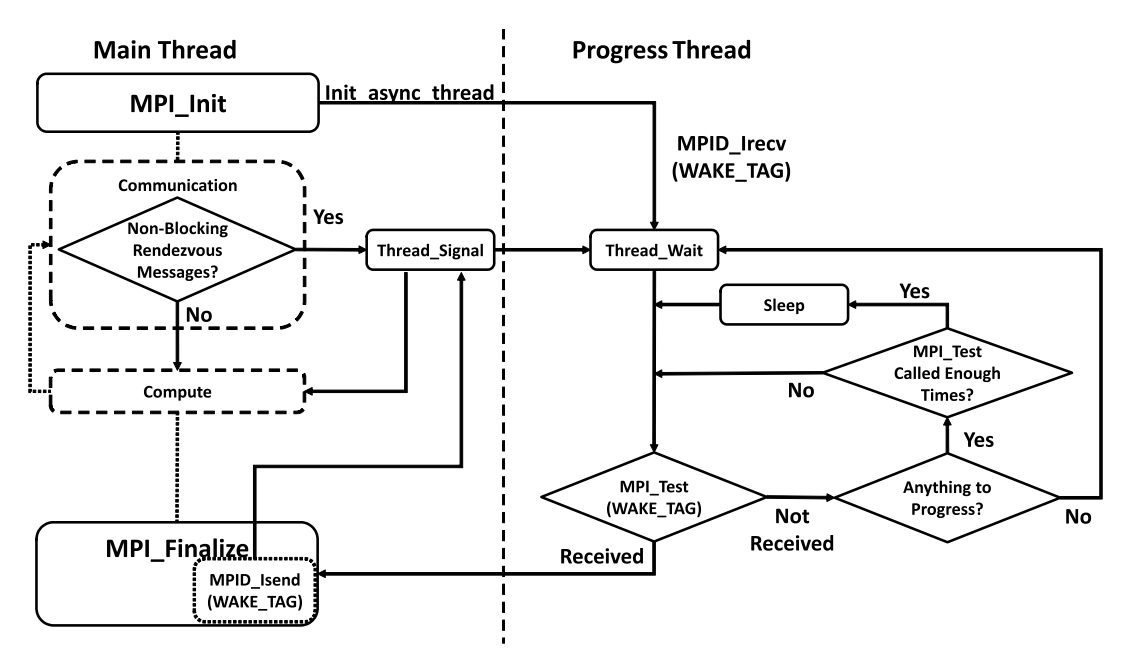
\includegraphics[width=0.8\linewidth]{TexFiles/Figures/Dummy-Diagram.png}
	\caption{Dummy Diagram, adapted from a dummy reference \cite{Li2020}}
	\label{fig:Dummy-Figure}
\end{figure}

\section{A section related to background}
\label{sec-bg-programming-models}

\lipsum[2-4]

\section{A more detailed subsection related to background}

\lipsum[5-6]

Let's have two figures, side by side in Figure \ref{fig:Side-by-Side-Figure}.
You can figure subfigures by \ref{fig:left-sub-figure} and \ref{fig:right-sub-figure}.

\begin{figure}
	\centering
	\begin{subfigure}[b]{0.45\linewidth}
		\centering
		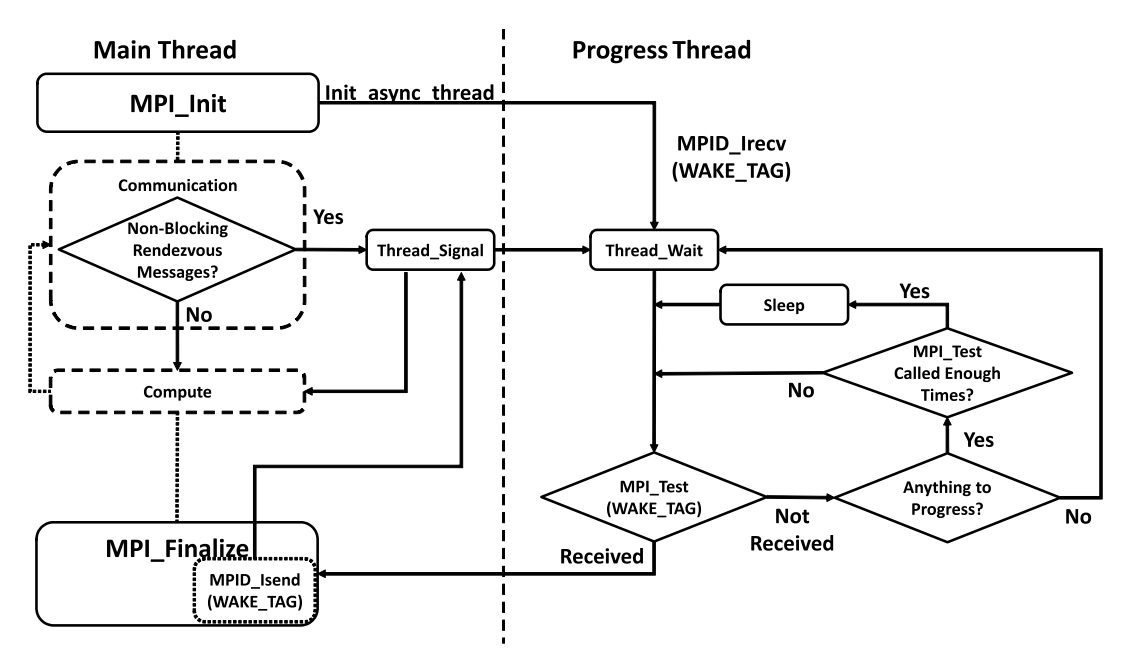
\includegraphics[width=\linewidth]{TexFiles/Figures/Dummy-Diagram.png}
		\caption{Same diagram as before!}
		\label{fig:left-sub-figure}
	\end{subfigure}
	\begin{subfigure}[b]{0.45\linewidth}
		\centering
		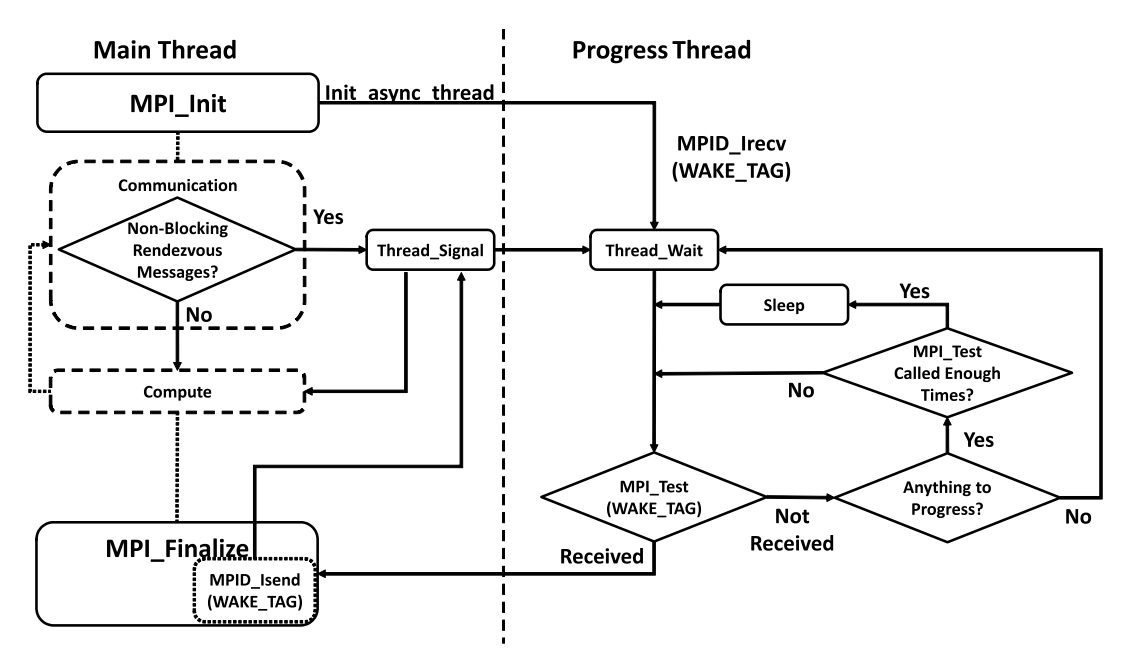
\includegraphics[width=\linewidth]{TexFiles/Figures/Dummy-Diagram.png}
		\caption{Same diagram as before, again!}
		\label{fig:right-sub-figure}
	\end{subfigure}
	\caption{Let's have the Same diagram as before, side by side!}
	\label{fig:Side-by-Side-Figure}
\end{figure}

\textbf{Important thing:} \lipsum[7-7]
%% ---------------------------------------------------------------
%% OnGoing Research
%% (C) AmirHossein Sojoodi @ Queen's University - 2020
%% ---------------------------------------------------------------

\chapter{Current State of Research}
\label{ch-research}

\lipsum[1-1]

%% ---------------------------------------------------------------
%% Research Directions
%% (C) AmirHossein Sojoodi @ Queen's University - 2020
%% ---------------------------------------------------------------

\section{First Research Direction}
\label{sec-first}

\lipsum[2-4]

Let's recall some acronyms: \gls{HPC}, \gls{MPI}, and \gls{CUDA}.

\subsection{Subsection related to first research direction}

\lipsum[1-1]
%% ---------------------------------------------------------------
%% Research Directions
%% (C) AmirHossein Sojoodi @ Queen's University - 2020
%% ---------------------------------------------------------------

\section{Second Research Direction}
\label{sec-second}

\lipsum[2-4]
Let's cite a reference here \cite{Bayatpour2020}. Let's cite several references together \cite{Bayatpour2020, Chu2020, Li2020, nvidiaweb}. 

\subsection{Subsection related to second research direction}

\lipsum[1-1]
%% ---------------------------------------------------------------
%% Conclusion
%% (C) AmirHossein Sojoodi @ Queen's University - 2020
%% ---------------------------------------------------------------

\chapter{Conclusion and Future Directions}
\label{ch-conclusion}

\lipsum[9-10]

%% ---------------------------------------------------------------
%% References
%% ---------------------------------------------------------------

% Print all the references:
% \nocite{*}

\KOMAoptions{fontsize=10.2pt}

%\setlength{\parskip}{0.5em}
\begin{spacing}{0.999}
\printbibliography[heading=bibintoc, title={References}]
\end{spacing}

%% ---------------------------------------------------------------
%% Appendix
%% ---------------------------------------------------------------

\appendix
% \input{Tex/appendix}

%% ---------------------------------------------------------------
%% End of the document
%% ---------------------------------------------------------------

\end{document}
